%% ------------- Portuguese version ------------
\documentclass{weciq}
\usepackage[english,brazil]{babel}
\usepackage[utf8]{inputenc}
\usepackage{amsmath}
\usepackage{graphicx}
\usepackage{threeparttable}
\usepackage{etoolbox}
\newtheorem{theorem}{Teorema}
%% ---------------------------------------------

%% If writing in English, remove the lines above
%% and uncomment the lines below

%% ------------- English version ---------------
%\documentclass[english]{sbrt}
%\usepackage[english]{babel}
%\usepackage[utf8]{inputenc}
%\newtheorem{theorem}{Theorem}
%% ---------------------------------------------

%% CONFIGURAÇÃO PARA VERSÃO ANÔNIMA
%% Descomente a linha abaixo para gerar versão anônima
%\newcommand{\anonversion}{}

\begin{document}

\newcommand{\weciqwcq}{VIII $\left<\right.$WECIQ$|$WCQ$\left.\right>$}

\title{Otimização de Arranjo de Turbinas Eólicas com QAOA considerando Efeitos de Esteira: Implementação com Qiskit}

\ifdef{\anonversion}{
  \author{Autor Anônimo}
}{
  \author{Marcos Vin\'icius C\^andido Henriques
  \thanks{Universidade Federal Rural do Semi-\'Arido (UFERSA), Campus Angicos, Departamento de Ci\'encias Exatas e Tecnologia da Informa\c{c}\~{a}o (DCETI). E-mail: viniciuscandido@ufersa.edu.br}%
  }
}

\maketitle

\markboth{VIII Workshop-Escola de Computação e Informação Quântica \& VIII Workshop de Computação Quântica - UFSC, 08--12 de Dezembro de 2025, Florianópolis, SC}{}


%% If writing in English, remove both 'resumo' and 'chave'
%% ------------- Portuguese version ------------
\begin{resumo}
Apresentamos uma formulação variacional para otimização do layout de turbinas eólicas em grades discretas considerando efeitos de esteira. O problema é modelado como QUBO que maximiza benefícios de cada posição e penaliza interações a jusante com decaimento por distância, mapeado para um Hamiltoniano compatível com QAOA. Demonstramos a penalização seletiva do estado $|11\rangle$ em pares sob esteira e realizamos experimentos numéricos em grades pequenas discutindo o compromisso entre ganho individual e penalidades de interferência, bem como limitações e perspectivas de escalabilidade.
\end{resumo}
\begin{chave}
QAOA, QUBO, fazendas eólicas, efeito de esteira, Qiskit, otimização combinatória.
\end{chave}
%% ---------------------------------------------


\begin{abstract}
We present a variational formulation for optimizing wind turbine layout on discrete grids under wake effects. The problem is modeled as a QUBO maximizing position benefits while penalizing downstream interactions with distance decay, mapped to a Hamiltonian suitable for QAOA. We demonstrate a selective $|11\rangle$ penalty on affected pairs and report small-grid numerical experiments discussing the trade-off between local gains and wake penalties, as well as scalability considerations.
\end{abstract}
\begin{keywords}
QAOA, wind farm layout, wake effect, Qiskit, QUBO.
\end{keywords}


\section{Introdu\c{c}\~{a}o}

A energia eólica representa uma das principais fontes renováveis para a geração sustentável de eletricidade, com crescente participação na matriz energética global \cite{GWEC2017, IRENA2017}. A eficiência dos parques eólicos depende significativamente do arranjo espacial das turbinas, uma vez que as interações aerodinâmicas entre elas, como o efeito de esteira, podem reduzir a produção energética total \cite{Jensen1983, Barthelmie2009}. Assim, a otimização do posicionamento das turbinas é um desafio relevante para maximizar a geração de energia e minimizar perdas. Recentemente, abordagens de computação quântica têm sido investigadas para este problema de otimização combinatória \cite{Kagemoto2024}.

Embora este trabalho seja inspirado no problema real de posicionamento de turbinas eólicas para mitigar perdas por esteira, o estudo aqui apresentado consiste em uma prova de conceito para a aplicação do algoritmo \textit{Quantum Approximate Optimization Algorithm} (QAOA) no ecossistema Qiskit para problemas de otimização formulados como \textit{Quadratic Unconstrained Binary Optimization} (QUBO).

O problema é modelado como um QUBO que visa maximizar o \textit{score} de produção e penalizar perdas por esteira com decaimento por distância, além de incluir restrições sobre o número de turbinas instaladas. Implementamos a construção do Hamiltoniano de custo que penaliza apenas pares de turbinas instaladas a jusante, junto com o \textit{ansatz} parametrizado e a otimização clássica subsequente. Os exemplos apresentados consideram grades pequenas (2×3, 3×3 e 4×4) para fins de prova de conceito e validação metodológica. Essa abordagem demonstra o potencial do uso de algoritmos quânticos aproximados para problemas complexos de otimização em energia renovável, servindo como base para trabalhos futuros.

\section{Metodologia}
\subsection{Formula\c{c}\~{a}o do problema}
Modelamos um grid de $R\times C$ posições. Cada variável binária $x_i\in\{0,1\}$ indica a presença de turbina na posição $i$. Um vetor $\{s_i\}$ atribui o benefício de cada posição. 

Para simplificação e como prova de conceito, os efeitos de esteira são codificados por uma matriz esparsa de penalidades $\{w_{ij}\}_{i<j}$ que decai linearmente com a distância discreta na mesma linha/coluna, respeitando uma regra direcional (p.ex., oeste\,$\rightarrow$\,leste ou norte\,$\rightarrow$\,sul). Esta aproximação linear é consideravelmente mais simples que modelos físicos realistas como Jensen \cite{Jensen1983} ou Gaussian \cite{Barthelmie2009}, que consideram decaimento não-linear, propagação radial da esteira, e efeitos de turbulência atmosférica.

Seja $G=(V,\mathcal{W})$ o grafo de conflitos, com $V=\{0,\dots,n-1\}$ e $\mathcal{W} = \{(i,j) \mid i<j, w_{ij}>0\}$ definindo pares de posições sob efeito de esteira.
Definimos benefício e penalidade clássicos
\begin{equation}
  B(x) \,=\, \sum_{i\in V} s_i\,x_i,\qquad
  P(x) \,=\, \sum_{(i,j)\in\mathcal{W}} w_{ij}\, x_i x_j,
\end{equation}
e otimizamos o custo (formulação QUBO; ver \cite{Kochenberger2014, Glover2018})
\begin{equation}
  C(x) \,=\, -\,B(x)\; +\; P(x) \quad \text{(a minimizar)},
\end{equation}
equivalente a maximizar $\sum_i s_i x_i - \sum_{(i,j)} w_{ij} x_i x_j$.

\subsection{Hamiltoniano de custo}
Usando o mapeamento $x_i = \frac{1 - Z_i}{2}$, escrevemos o Hamiltoniano de custo (forma de Pauli-Z):
\begin{equation}
  H_C \,=\, - \sum_{i\in V} s_i\, \frac{1 - Z_i}{2}\; +\; \sum_{(i,j)\in\mathcal{W}} w_{ij}\, \frac{(1 - Z_i)(1 - Z_j)}{4}.
\end{equation}
Os termos elementares são
\begin{align}
  H^{(1)}_i &= -\frac{s_i}{2}\,\big(I - Z_i\big), \\
  H^{(2)}_{ij} &= \frac{w_{ij}}{4}\,\big( Z_i Z_j - Z_i - Z_j + I \big) \;\equiv\; \frac{w_{ij}}{4}\,(1 - Z_i)(1 - Z_j),
\end{align}
garantindo que apenas o estado $|11\rangle$ do par $(i,j)$ é penalizado por $w_{ij}$. Aqui, $Z_i$ representa o operador de Pauli-Z atuando no qubit $i$, e o produto tensorial $Z_iZ_j = Z_i \otimes Z_j$ permite detectar quando ambas as posições $i$ e $j$ possuem turbinas instaladas (estado $|11\rangle$), condição necessária para que ocorra interferência de esteira entre elas.

\subsection{QAOA e formalismo}
Adotamos o misturador e o estado inicial usuais
\begin{equation}
  H_M \,=\, \sum_{i\in V} X_i,\qquad |\psi_0\rangle \,=\, |+\rangle^{\otimes n},
\end{equation}
com operadores de evolução por camada
\begin{equation}
  U_C(\gamma) \,=\, e^{-i\,\gamma\, H_C},\qquad U_M(\beta) \,=\, e^{-i\,\beta\, H_M}.
\end{equation}
O \textit{ansatz} de profundidade $p$ é (QAOA; \cite{Farhi2014,QiskitAlgorithms})
\begin{equation}
  |\psi(\boldsymbol{\gamma},\boldsymbol{\beta})\rangle \,=\, U_M(\beta_p)\,U_C(\gamma_p)\,\cdots\,U_M(\beta_1)\,U_C(\gamma_1)\,|\psi_0\rangle,
\end{equation}
e os parâmetros $\{\gamma_\ell,\beta_\ell\}_{\ell=1}^p$ são otimizados por rotina clássica visando minimizar $\langle H_C\rangle$.

\subsection{Configuração experimental}
Implementamos a solução utilizando o \textit{framework} Qiskit 2.1.0 \cite{QiskitCommunity2017} com simulador AER para execução dos circuitos quânticos. O simulador AER (Aer \textit{Quantum Simulator}) fornece simulação clássica de alta performance dos circuitos QAOA (ver exemplo na Fig.~6), permitindo execução eficiente com controle de paralelismo. Os experimentos são configuráveis através de parâmetros que especificam: (i) dimensões da grade ($R \times C$); (ii) direção do vento representada por vetor unitário; (iii) distribuição dos \textit{score}s $s_i$ (valores fixos, uniformes ou aleatórios); (iv) parâmetros de penalidade máxima e fator de decaimento; (v) configurações do QAOA (número de camadas $p$, iterations, optimizador); e (vi) restrições de cardinalidade sobre o número de turbinas.

Para garantir reprodutibilidade, utilizamos sementes fixas (seed=42) na geração de \textit{score}s aleatórios. O otimizador COBYLA foi empregado, executando até 200 iterações ou convergência, com parâmetro \texttt{rhobeg} (raio inicial da região de confiança) variando conforme o experimento. O número de shots foi fixado em 1024 para estimativas estatísticas confiáveis das expectativas. Todas as simulações foram executadas em CPU utilizando o simulador Qiskit AER com controle do número de threads paralelas via parâmetro \texttt{max\_parallel\_threads}. A máquina utilizada possui processador Intel Core i3-10100 (4 cores, 8 threads, 3.6 GHz base / 4.3 GHz boost) e 8 GB de RAM, executando Ubuntu 22.04 LTS.

\section{Resultados num\'ericos}
Apresentamos resultados para grades pequenas (2x3, 3x3, 4x4) sob direções de vento fixas utilizando simulação clássica através do simulador Qiskit AER \cite{QiskitCommunity2017}. As métricas de interesse incluem: (i) valor esperado de $H_C$ ao final da otimização, (ii) probabilidade da melhor solução encontrada, (iii) benefício líquido (\textit{score} total menos penalidade de esteira), (iv) cardinalidade da solução, e (v) razão de penalidade (fração de pares penalizados). 

O QAOA demonstra capacidade de capturar o \emph{trade-off} entre maximizar benefícios individuais e minimizar interferências de esteira. A convergência é sensível aos pesos $s_i$ e $w_{ij}$, à profundidade $p$ do \textit{ansatz}, e à inicialização dos parâmetros variacionais. Grades maiores apresentam desafios de escalabilidade na simulação em computação clássica, devido ao crescimento exponencial do número de estados possíveis.

\subsection*{Exemplo de simula\c{c}\~{a}o \textit{single-run}}
Apresentamos, para ilustração, três artefatos de uma única execução representativa: evolução do custo, trajetória dos parâmetros e layout final estimado.

\begin{figure}[htb]
\centering
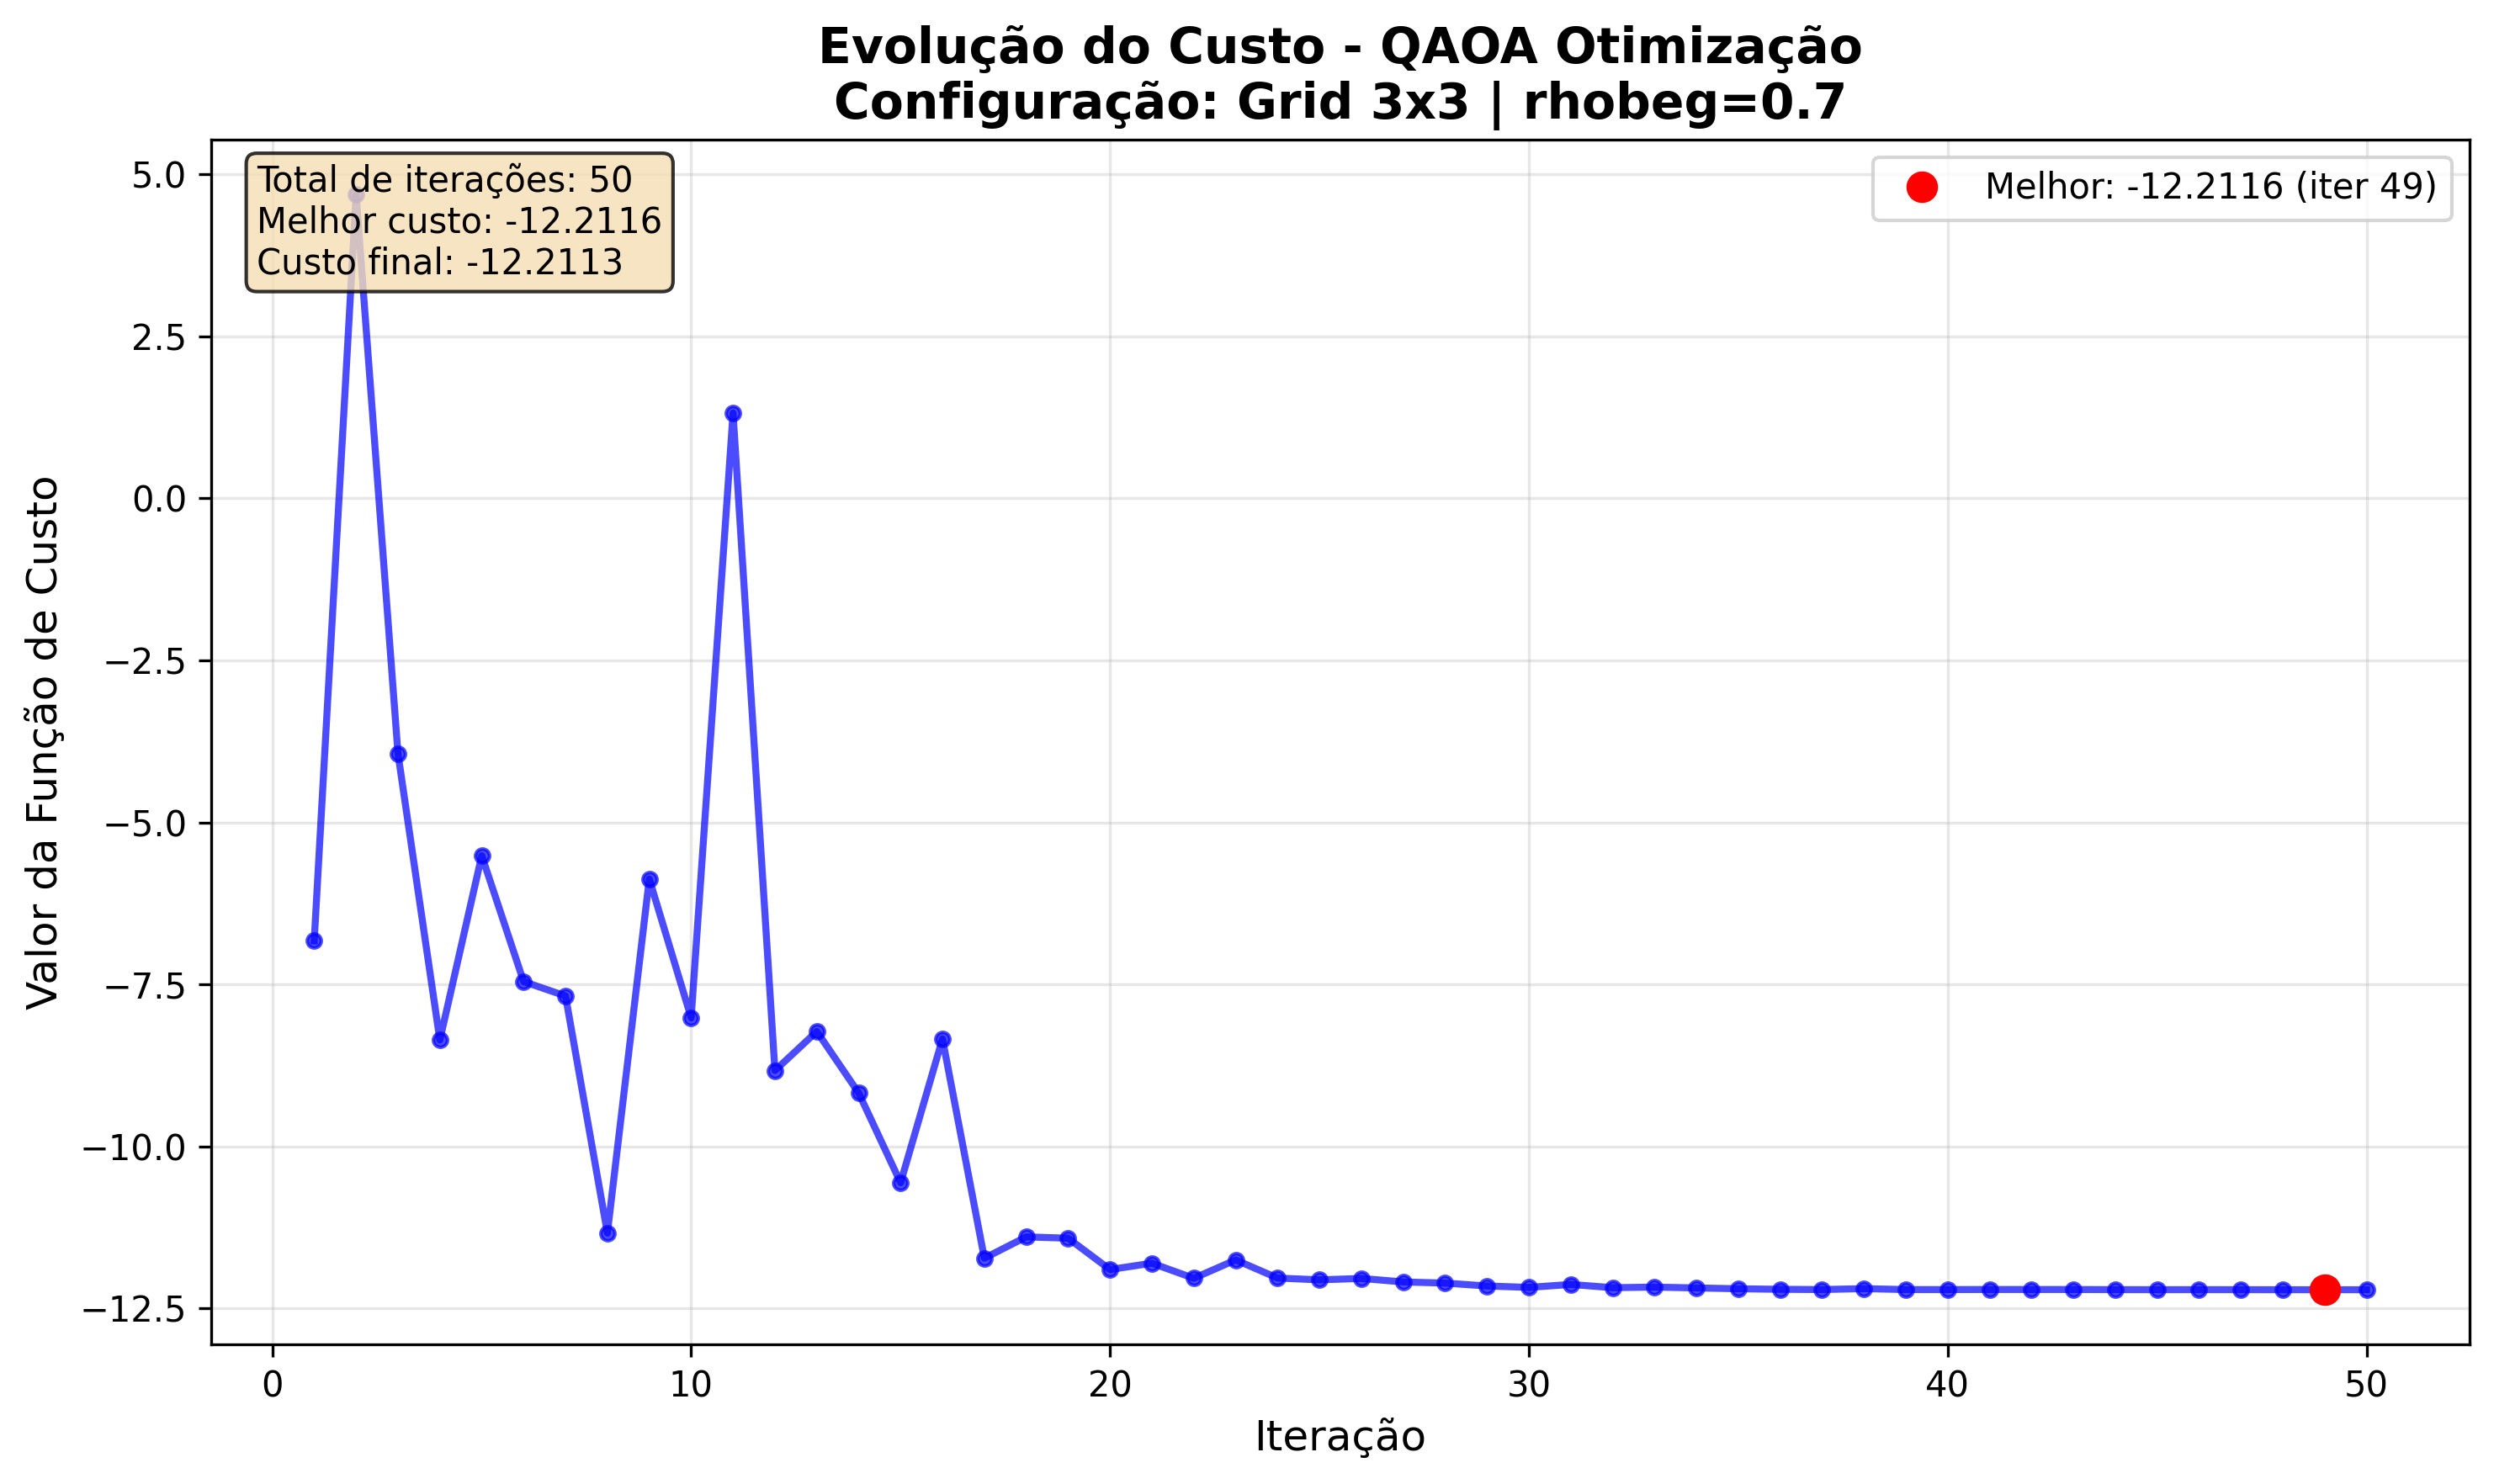
\includegraphics[width=0.95\linewidth]{iteracoes.png}
\caption{Evolução do valor esperado de $H_C$ ao longo das iterações da otimização clássica para uma grade 3x3, demonstrando o processo de convergência do algoritmo QAOA.}
\end{figure}

\begin{figure}[htb]
\centering
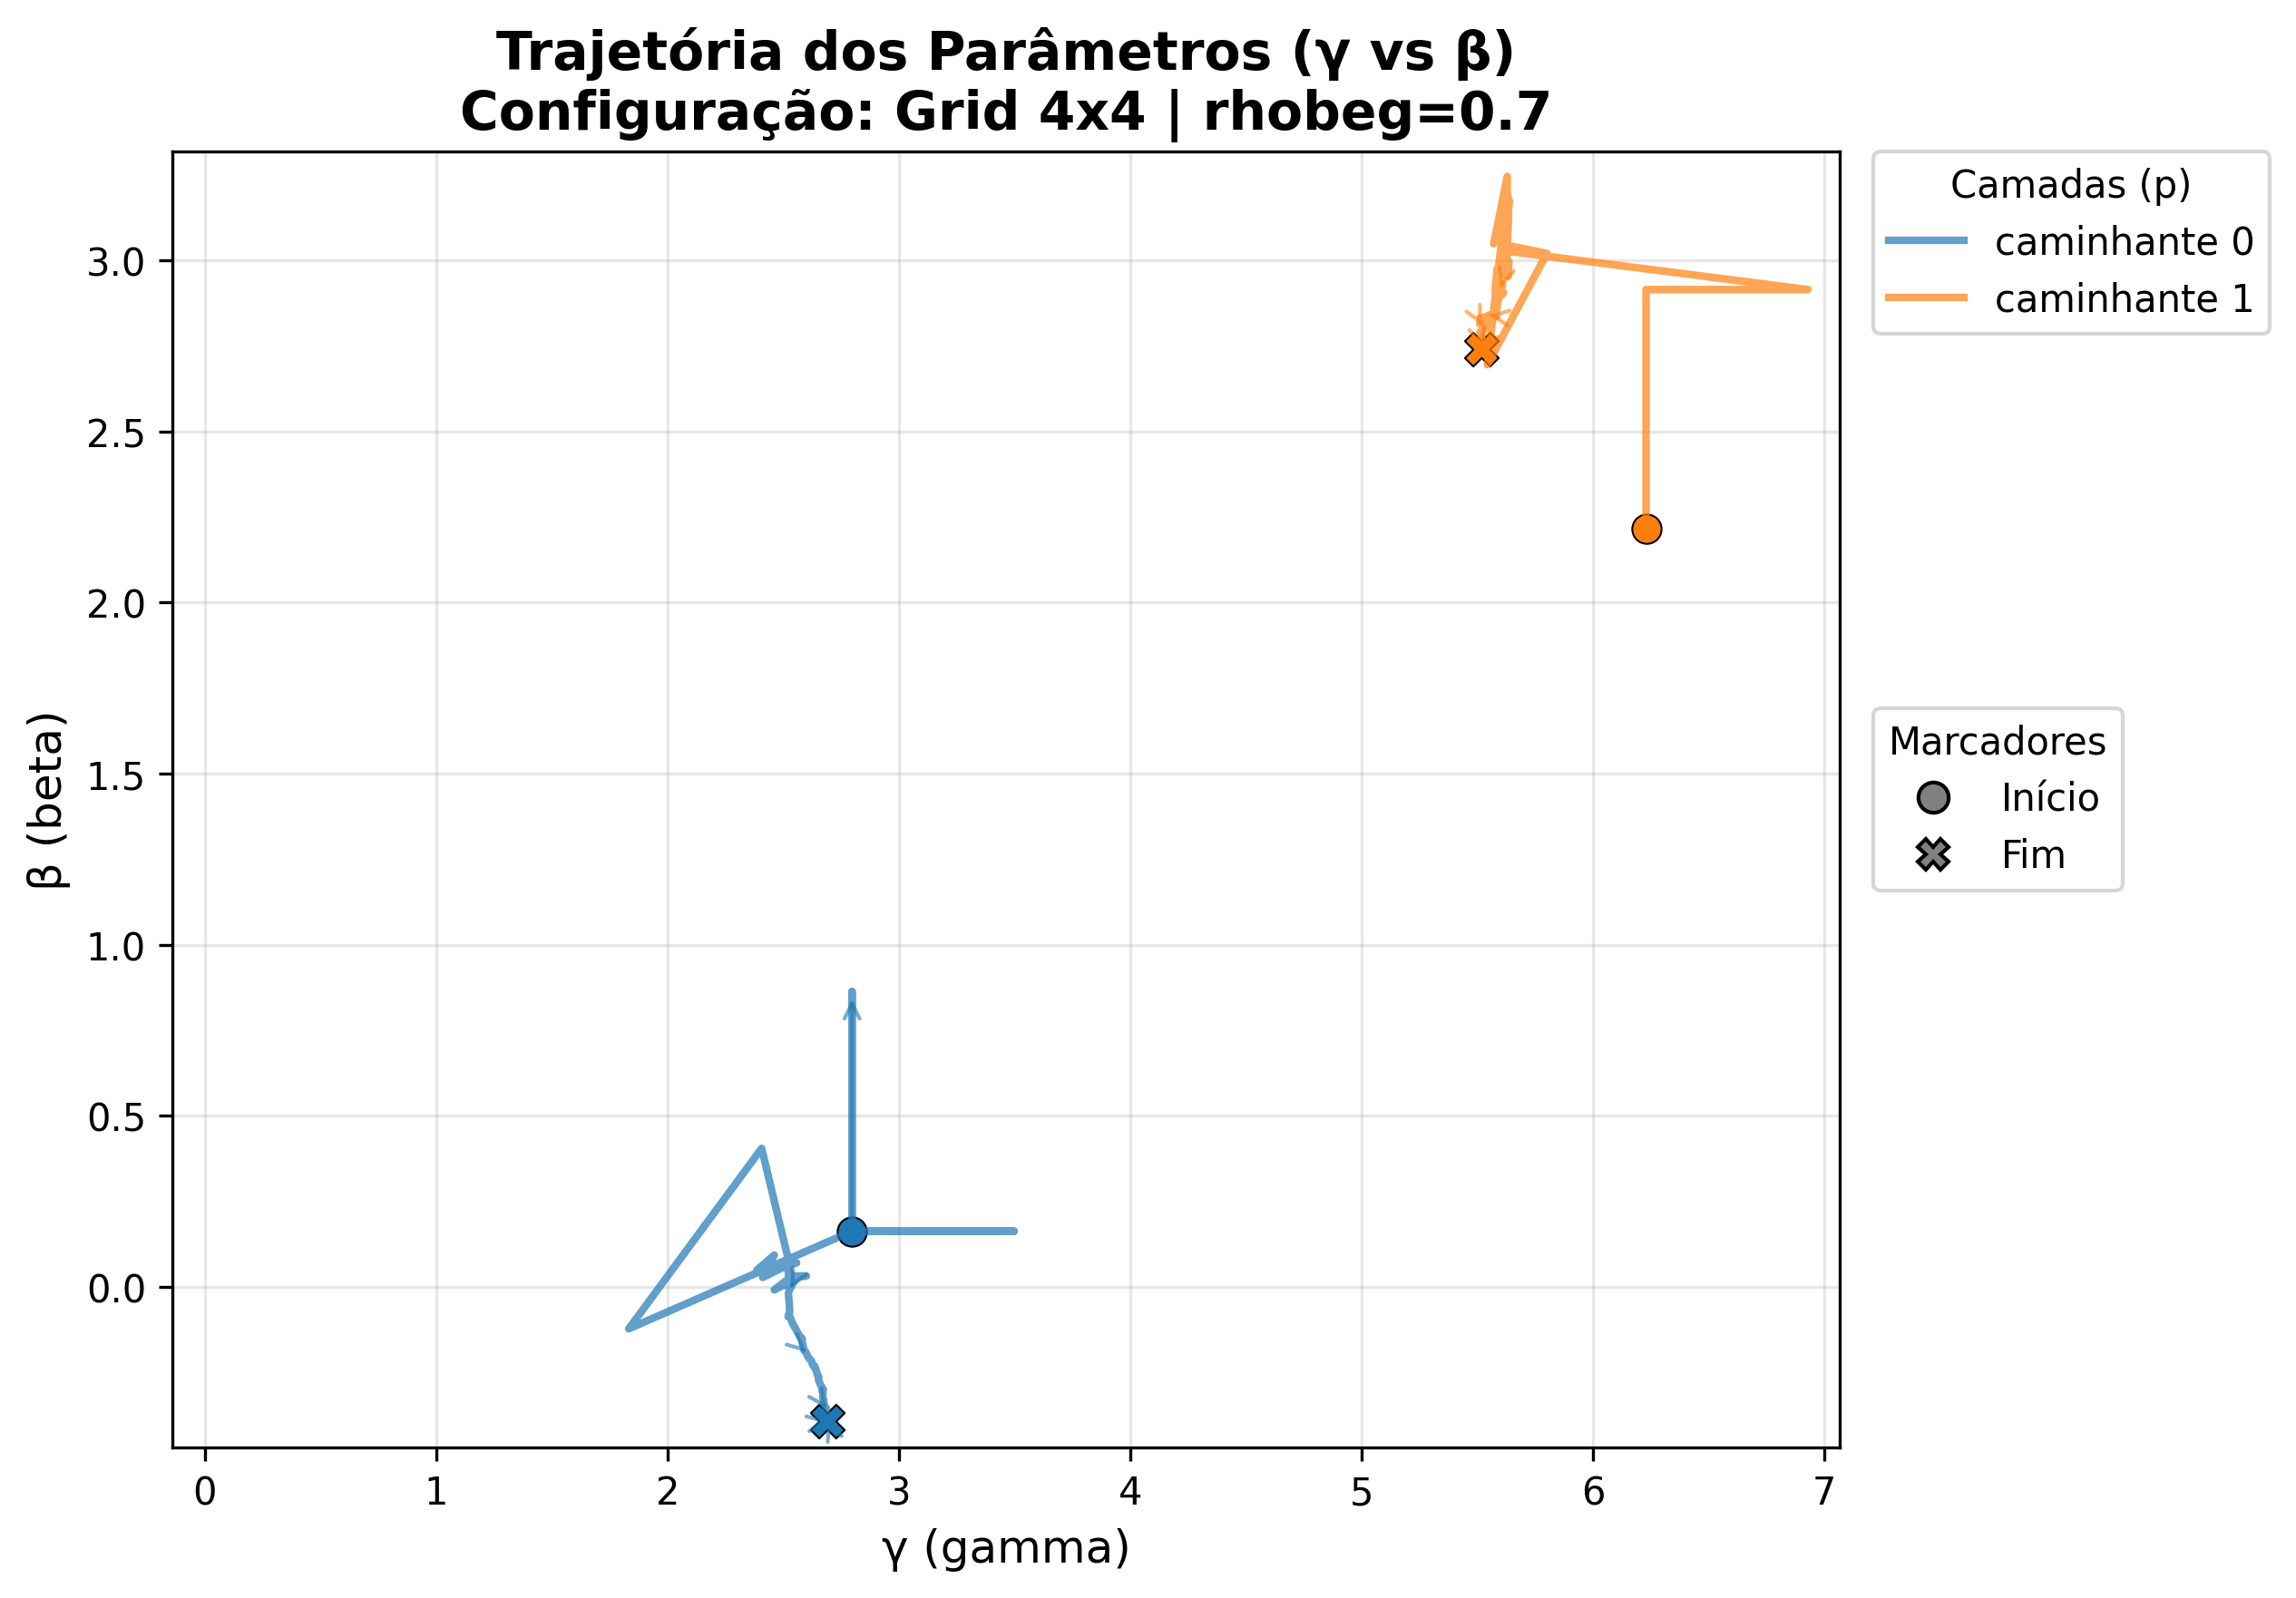
\includegraphics[width=0.95\linewidth]{trajetoria.png}
\caption{Trajetória dos parâmetros $(\gamma,\beta)$ por camada ao longo do processo variacional para grade 3x3 com duas camadas QAOA. Observa-se a exploração do espaço de parâmetros com convergência estável, onde os valores finais balanceiam a influência do Hamiltoniano de custo ($\gamma$) e do operador de mistura ($\beta$).}
\end{figure}

\subsection*{Exemplos por dimens\~{a}o de grade}
Os layouts a seguir ilustram soluções otimizadas encontradas pelo QAOA para diferentes dimensões de grade, evidenciando estratégias distintas de posicionamento.

\begin{figure}[htb]
\centering
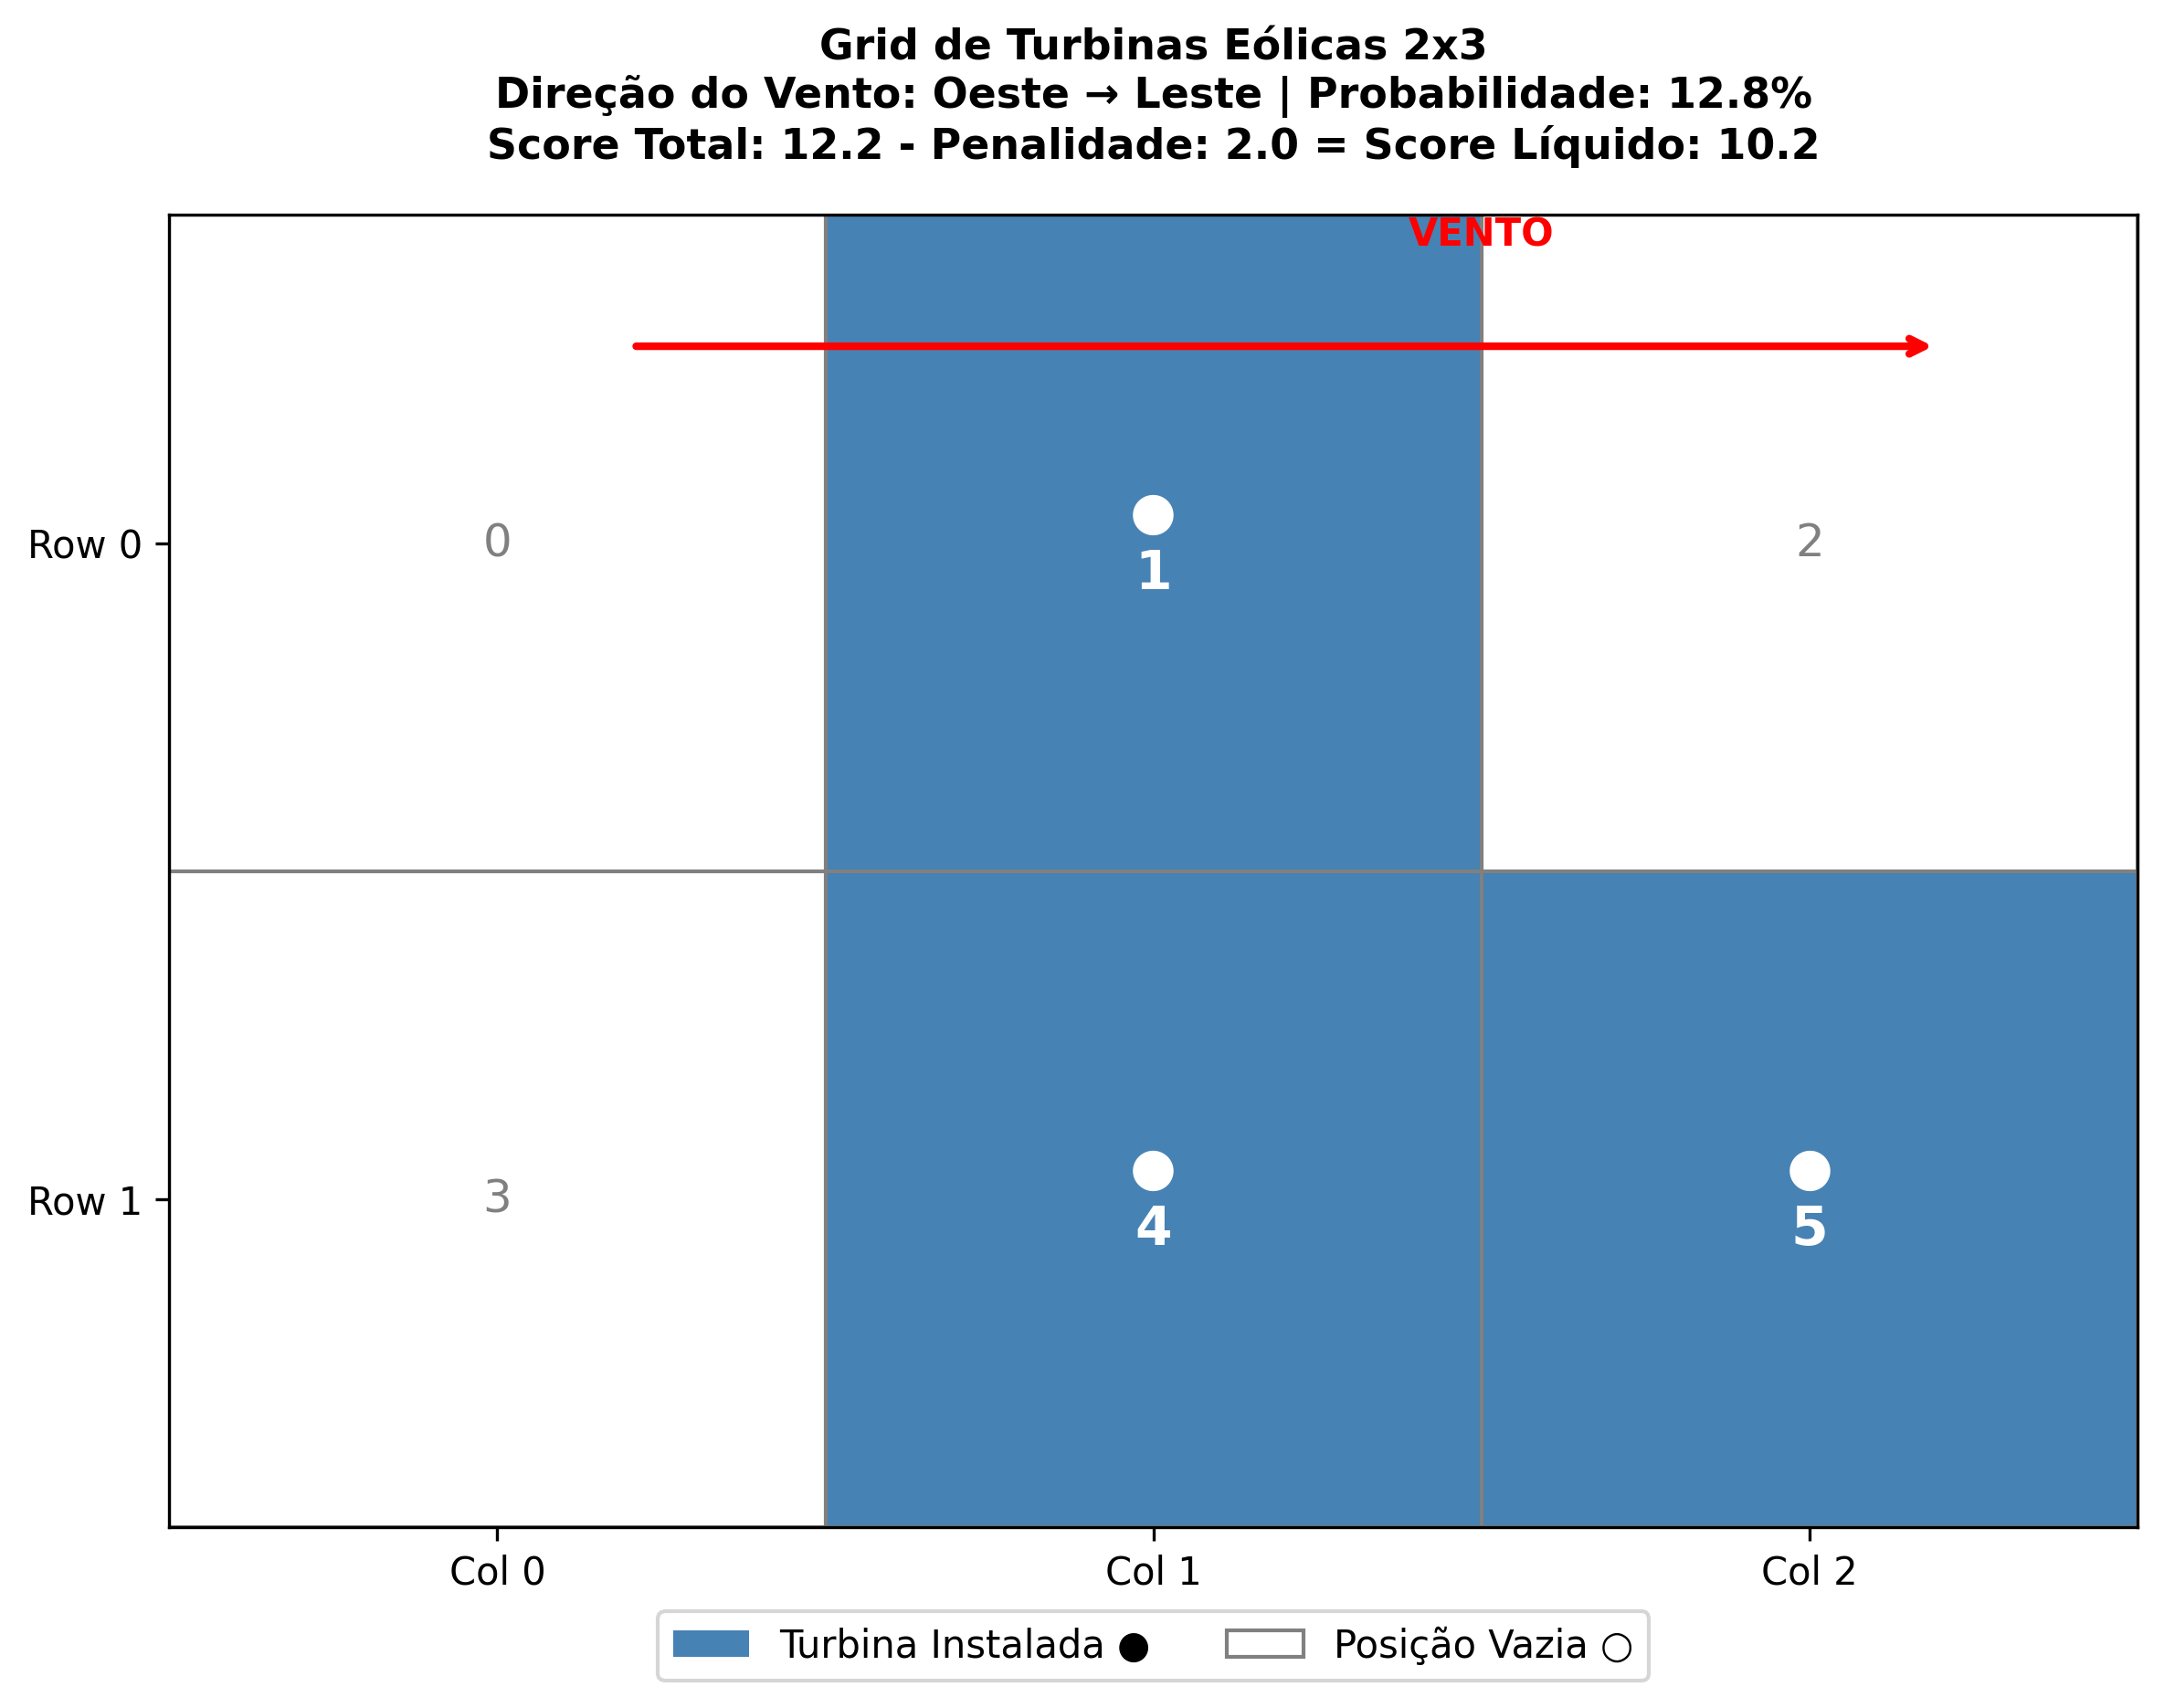
\includegraphics[width=0.85\linewidth]{grid_visualization_default_2x3_3turbinas_20250810_144135.png}
\caption{Resultado otimizado pelo QAOA para grade 2x3 (configuração binária 010011), com 3 turbinas instaladas. Esta solução não é globalmente ótima, apresentando penalidade de esteira entre as turbinas das posições (1,1) e (1,2), onde uma turbina está diretamente a jusante da outra na direção oeste-leste do vento.}
\end{figure}

\begin{figure}[htb]
\centering
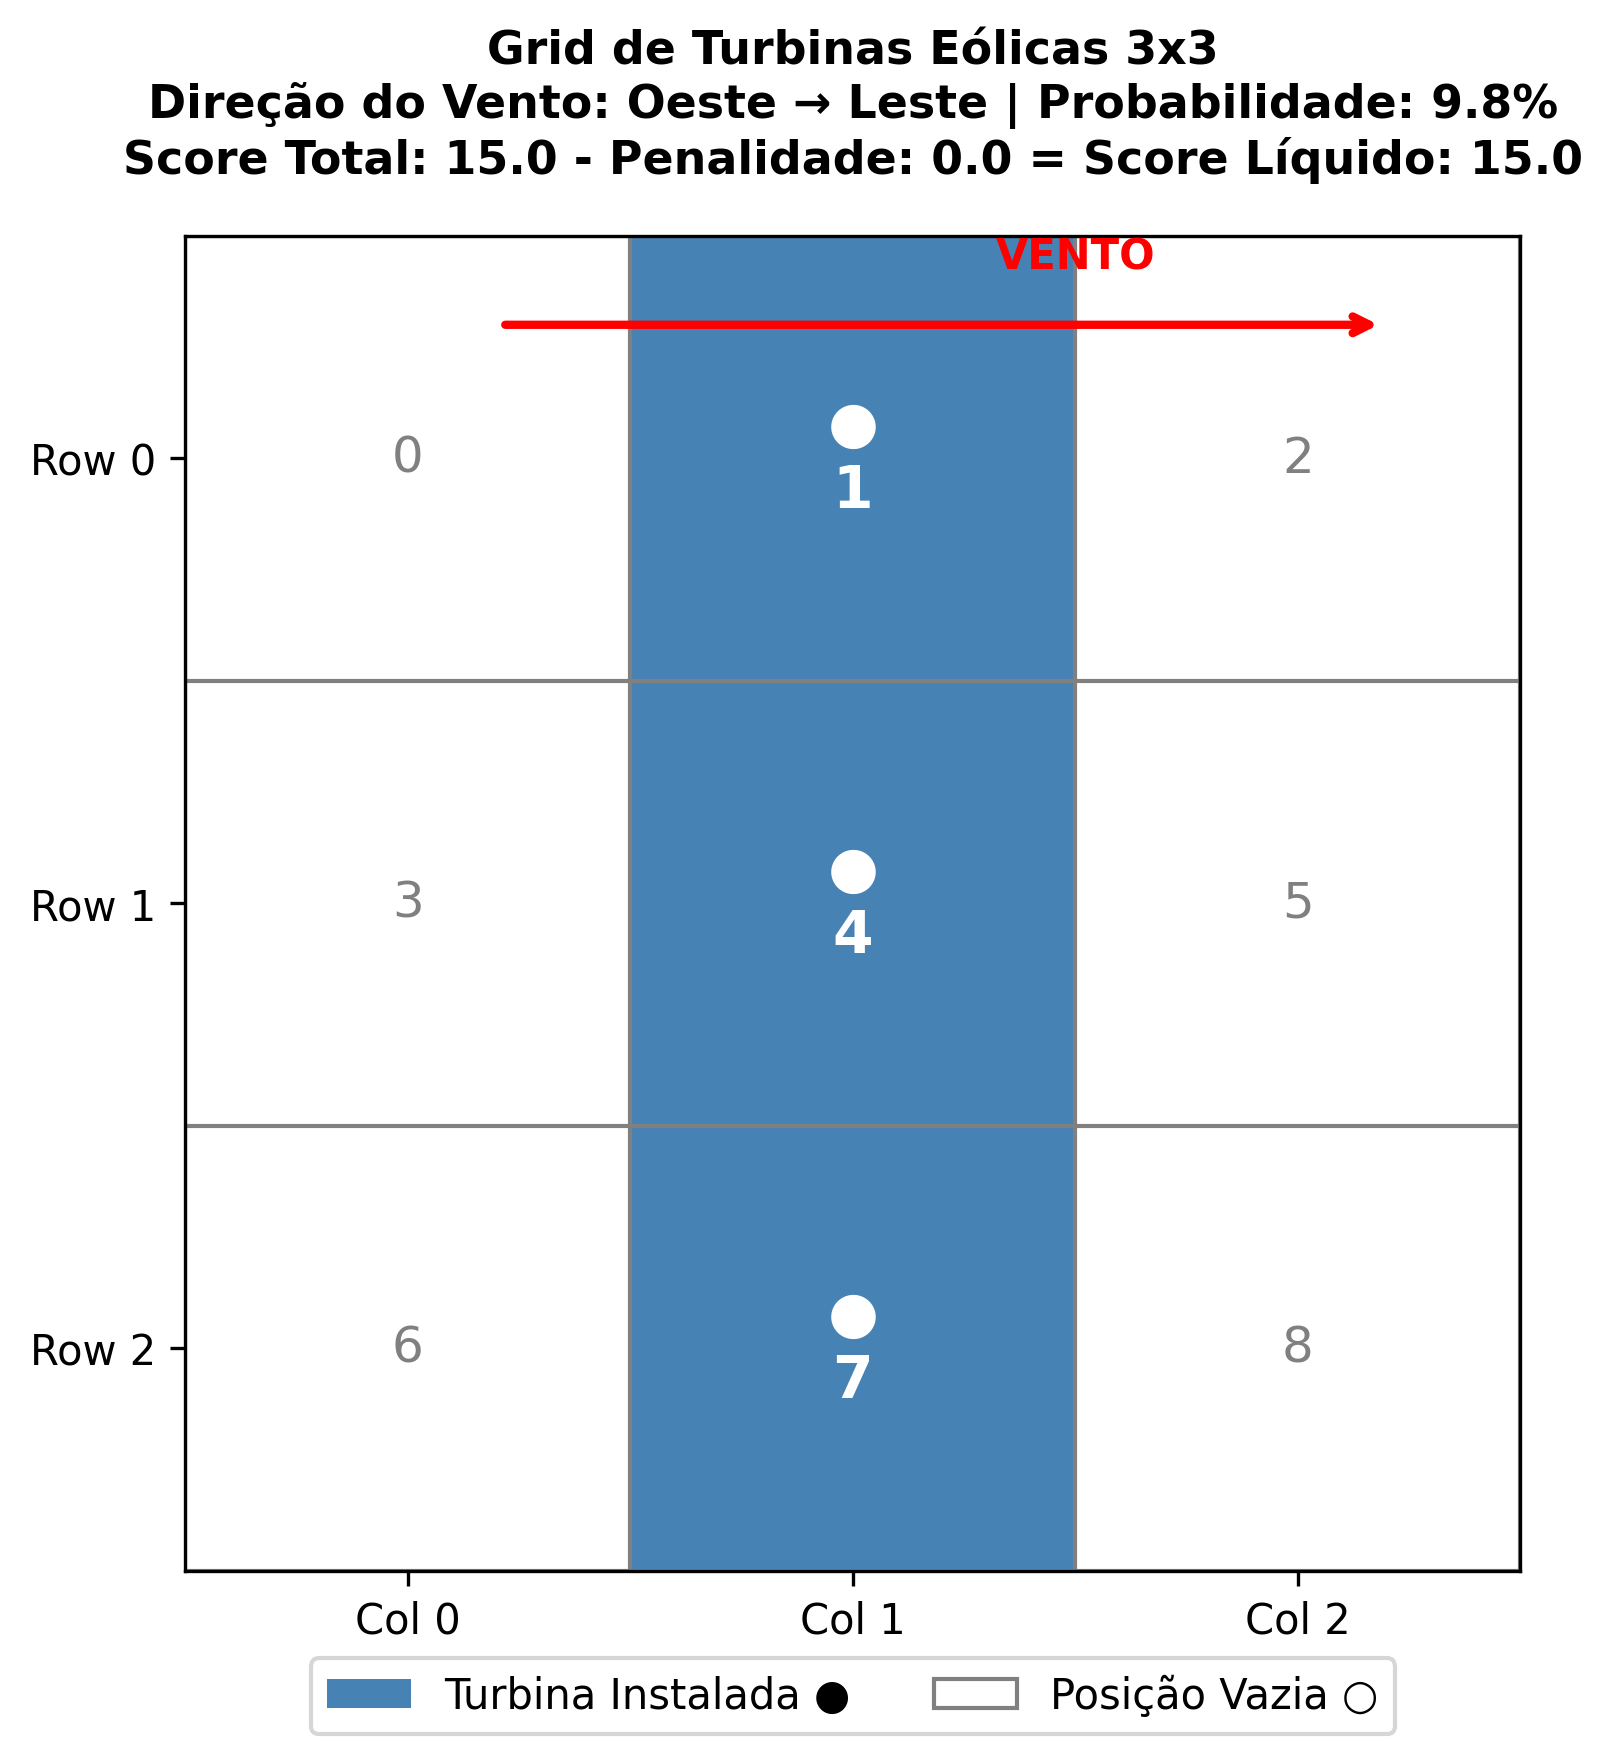
\includegraphics[width=0.85\linewidth]{grid_visualization_temp_3x3_p2_rhobeg0.5_rep2_3x3_3turbinas_20250820_205303.png}
\caption{Layout otimizado para grade 3x3 com QAOA (p=2, rhobeg=0.5), mostrando distribuição estratégica de 3 turbinas nas posições (0,1), (1,1) e (2,1), todas na coluna central, eliminando completamente interferências de esteira.}
\end{figure}

\begin{figure}[h!]
\centering
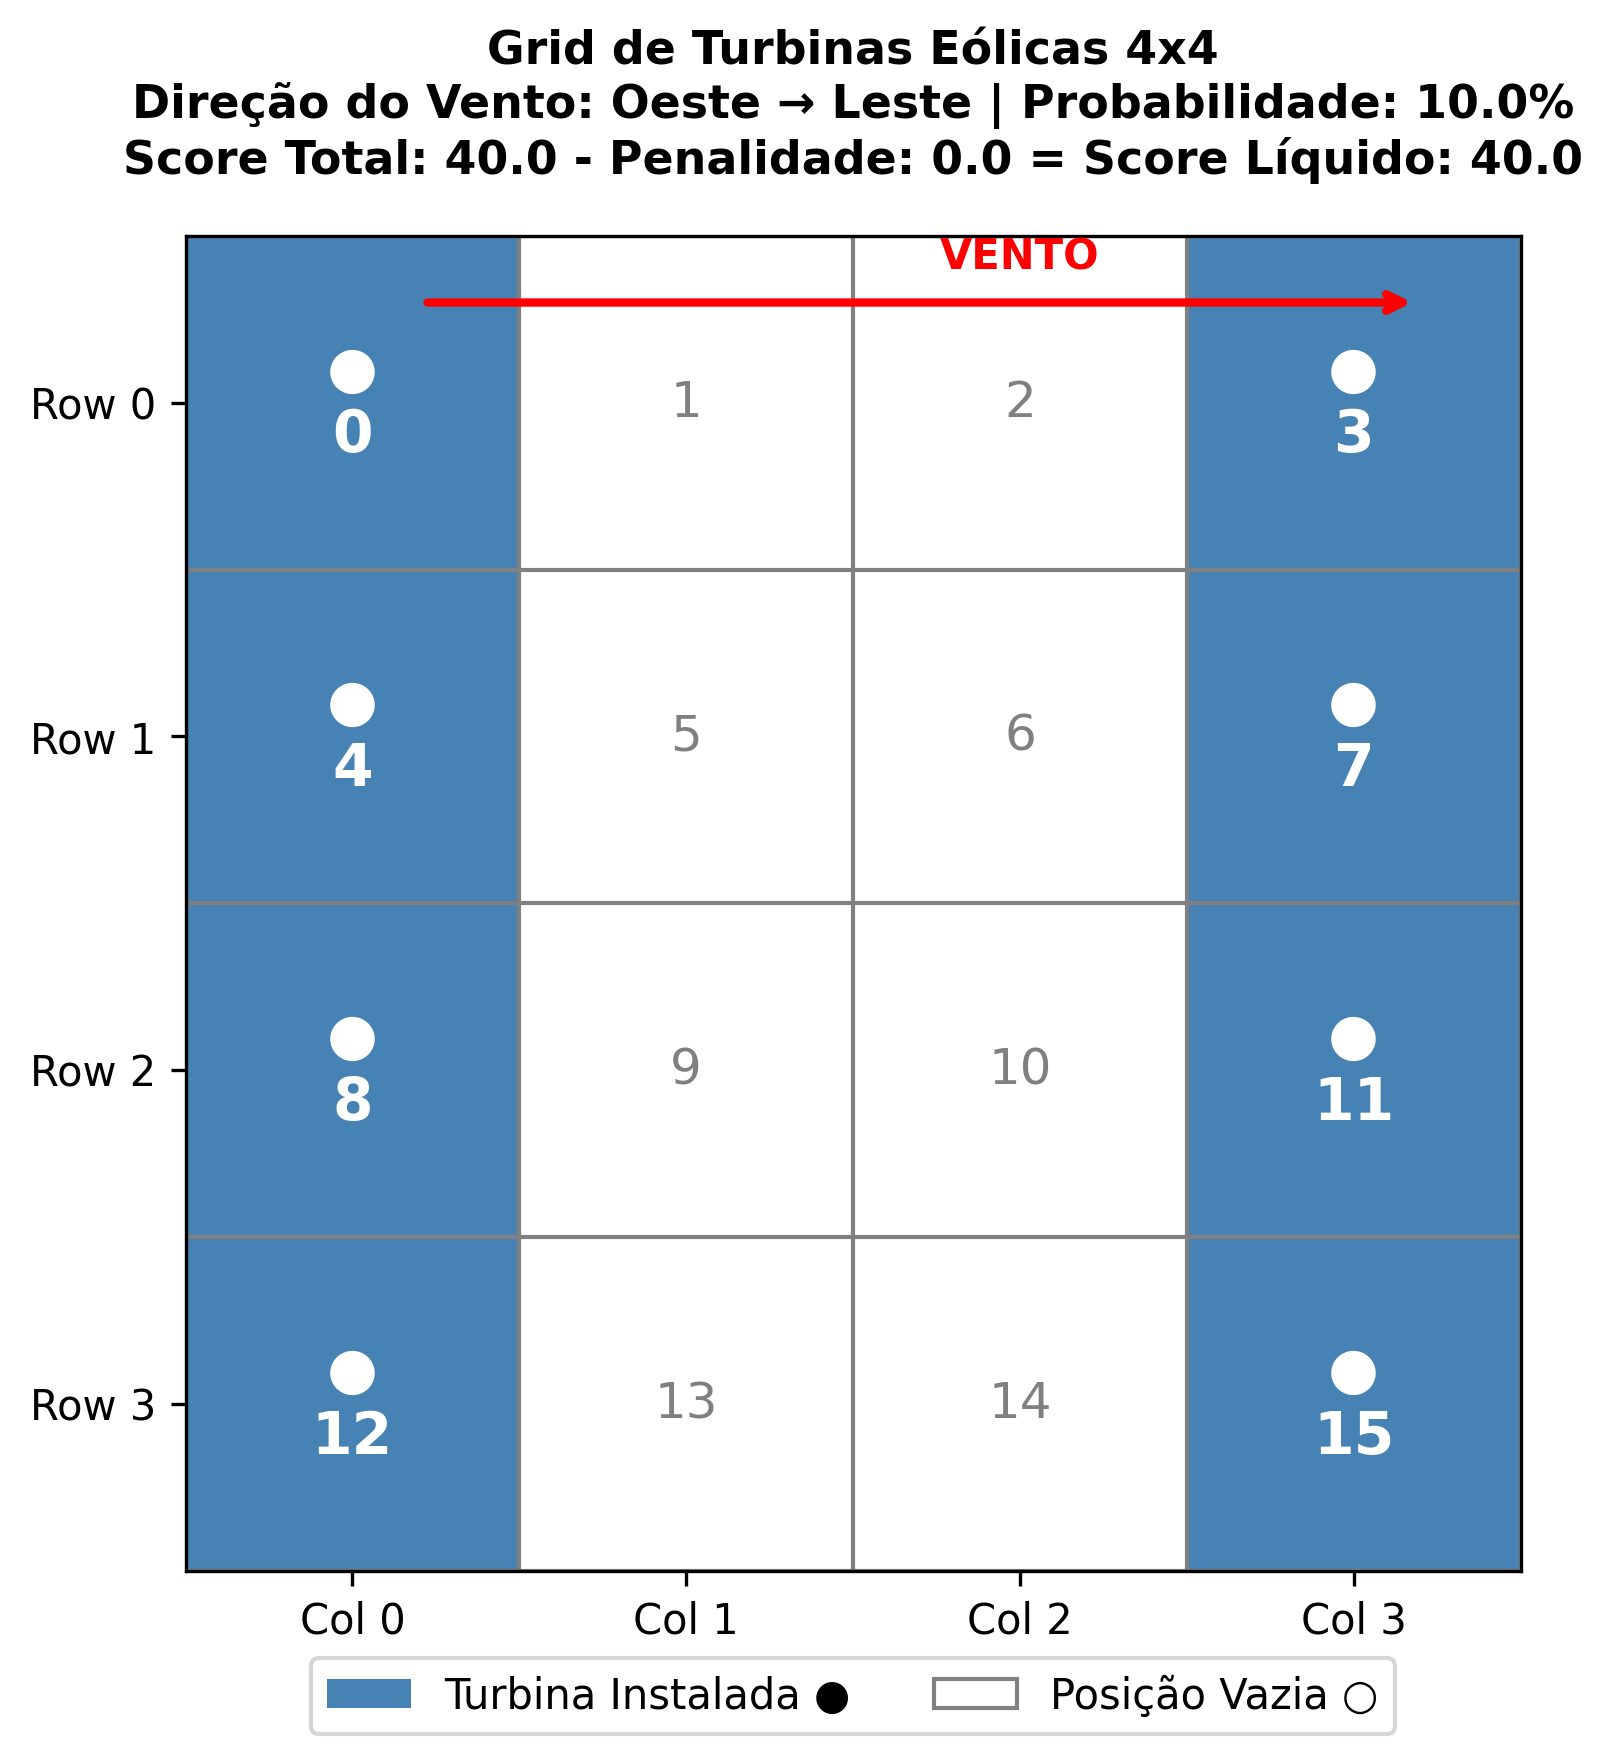
\includegraphics[width=0.85\linewidth]{grid_visualization_4x4_4x4_8turbinas_20250810_124433.png}
\caption{Layout otimizado para grade 4x4 com 8 turbinas organizadas em duas fileiras verticais nas colunas externas (0 e 3). Os parâmetros base\_penalty=12.0 e distance\_decay=4.0 foram escolhidos didaticamente para demonstrar que a solução ótima pode permitir alinhamentos de turbinas quando o benefício individual supera as penalidades de esteira calculadas.}
\end{figure}

\subsection*{Resultados Benchmarks Sistemáticos}

Os resultados apresentados a seguir foram obtidos através de benchmarks sistemáticos com 81 execuções totais, testando diferentes combinações de número de camadas QAOA (p=1, 2, 3) e valores do parâmetro \texttt{rhobeg} do otimizador COBYLA (0.3, 0.5, 0.7), com 3 repetições por configuração para maior confiabilidade estatística.

Os parâmetros de penalização de esteira utilizados para cada grid foram ajustados conforme a dimensão:
\begin{itemize}
\item \textbf{Grid 2x3}: base\_penalty = 3.0, distance\_decay = 1.0
\item \textbf{Grid 3x3}: base\_penalty = 8.0, distance\_decay = 1.0  
\item \textbf{Grid 4x4}: base\_penalty = 12.0, distance\_decay = 4.0
\end{itemize}

Estes valores foram escolhidos para fins didáticos, demonstrando diferentes cenários de otimização. No grid 4x4, em particular, o distance\_decay = 4.0 foi selecionado para permitir que a solução ótima contenha duas fileiras completas de turbinas nas colunas externas, evidenciando situações onde o benefício individual supera as penalidades de esteira mesmo com alinhamentos diretos.

\begin{table*}[htbp]
\centering
\caption{Resultados QAOA para Grid 2x3 (6 qubits) - Análise por Camadas e parâmetro rhobeg do COBYLA. Tempos de execução obtidos em processador Intel Core i3-10100.}
\label{tab:resultados_2_3}
\footnotesize
\begin{tabular}{|c|c|c|c|c|c|c|c|}
\hline
\textbf{Camadas} & \textbf{rhobeg (COBYLA)} & \textbf{Prob. Média (\%)} & \textbf{Prob. Máx (\%)} & \textbf{Score Médio} & \textbf{Score Máximo} & \textbf{Turbinas Médias} & \textbf{Tempo (s)} \\
\hline
1 & 0.3 & 32.7 & 71.0 & 18.3 & 20.0 & 4.7 & 0.62 \\
1 & 0.5 & 15.7 & 21.0 & 18.0 & 18.0 & 4.0 & 0.62 \\
1 & 0.7 & 11.0 & 12.0 & 12.0 & 17.0 & 2.7 & 0.61 \\
2 & 0.3 & 68.3 & 70.0 & 20.0 & 20.0 & 6.0 & 0.72 \\
2 & 0.5 & 39.0 & 96.0 & 19.7 & 20.0 & 5.7 & 0.82 \\
2 & 0.7 & 39.7 & 67.0 & 19.3 & 20.0 & 5.3 & 0.74 \\
3 & 0.3 & 56.3 & 96.0 & 19.7 & 20.0 & 5.7 & 0.87 \\
3 & 0.5 & 86.7 & 93.0 & 20.0 & 20.0 & 6.0 & 0.85 \\
3 & 0.7 & 52.3 & 65.0 & 20.0 & 20.0 & 6.0 & 0.81 \\
\hline
\end{tabular}
\end{table*}

\begin{table*}[htbp]
\centering
\caption{Resultados QAOA para Grid 3x3 (9 qubits) - Análise por Camadas e parâmetro rhobeg do COBYLA. Tempos de execução obtidos em processador Intel Core i3-10100.}
\label{tab:resultados_3_3}
\footnotesize
\begin{tabular}{|c|c|c|c|c|c|c|c|}
\hline
\textbf{Camadas} & \textbf{rhobeg (COBYLA)} & \textbf{Prob. Média (\%)} & \textbf{Prob. Máx (\%)} & \textbf{Score Médio} & \textbf{Score Máximo} & \textbf{Turbinas Médias} & \textbf{Tempo (s)} \\
\hline
1 & 0.3 & 4.3 & 5.0 & 10.0 & 11.0 & 5.0 & 0.70 \\
1 & 0.5 & 4.3 & 5.0 & 10.0 & 11.0 & 5.0 & 0.71 \\
1 & 0.7 & 4.3 & 5.0 & 11.7 & 15.0 & 4.0 & 0.67 \\
2 & 0.3 & 13.3 & 18.0 & 13.0 & 15.0 & 3.7 & 0.85 \\
2 & 0.5 & 10.0 & 18.0 & 13.0 & 15.0 & 3.0 & 0.85 \\
2 & 0.7 & 4.3 & 5.0 & 12.7 & 15.0 & 4.0 & 0.85 \\
3 & 0.3 & 12.0 & 13.0 & 13.0 & 15.0 & 3.0 & 0.95 \\
3 & 0.5 & 13.0 & 14.0 & 13.0 & 15.0 & 4.0 & 0.95 \\
3 & 0.7 & 5.0 & 7.0 & 13.7 & 15.0 & 3.3 & 0.97 \\
\hline
\end{tabular}
\end{table*}

\begin{table*}[htbp]
\centering
\caption{Resultados QAOA para Grid 4x4 (16 qubits) - Análise por Camadas e parâmetro rhobeg do COBYLA. Tempos de execução obtidos em processador Intel Core i3-10100.}
\label{tab:resultados_4_4}
\footnotesize
\begin{tabular}{|c|c|c|c|c|c|c|c|}
\hline
\textbf{Camadas} & \textbf{rhobeg (COBYLA)} & \textbf{Prob. Média (\%)} & \textbf{Prob. Máx (\%)} & \textbf{Score Médio} & \textbf{Score Máximo} & \textbf{Turbinas Médias} & \textbf{Tempo (s)} \\
\hline
1 & 0.3 & 2.0 & 2.0 & 20.7 & 30.0 & 7.3 & 3.28 \\
1 & 0.5 & 1.7 & 2.0 & 16.0 & 20.0 & 6.7 & 1.74 \\
1 & 0.7 & 1.7 & 2.0 & 16.7 & 17.0 & 6.7 & 1.48 \\
2 & 0.3 & 2.0 & 2.0 & 30.0 & 36.0 & 7.0 & 7.35 \\
2 & 0.5 & 1.3 & 2.0 & 6.3 & 13.0 & 8.3 & 14.29 \\
2 & 0.7 & 2.7 & 4.0 & 21.3 & 31.0 & 6.7 & 4.40 \\
3 & 0.3 & 3.7 & 7.0 & 35.3 & 40.0 & 7.3 & 14.82 \\
3 & 0.5 & 32.3 & 92.0 & 34.7 & 40.0 & 8.0 & 12.88 \\
3 & 0.7 & 2.3 & 3.0 & 26.3 & 40.0 & 7.7 & 13.35 \\
\hline
\end{tabular}
\end{table*}

\begin{table*}[htbp]
\centering
\caption{Comparação de Performance QAOA: Melhores Resultados por Grid. Tempos de execução obtidos em processador Intel Core i3-10100.}
\label{tab:benchmark_comparison}
\footnotesize
\begin{tabular}{|c|c|c|c|c|c|c|c|}
\hline
\textbf{Grid} & \textbf{Qubits} & \textbf{Score Máximo} & \textbf{Camadas Ótimas} & \textbf{rhobeg Ótimo (COBYLA)} & \textbf{Prob. Máx (\%)} & \textbf{Turbinas Médias} & \textbf{Tempo Médio (s)} \\
\hline
2x3 & 6 & 20.0 & 1 & 0.3 & 71.0 & 4.7 & 0.62 \\
3x3 & 9 & 15.0 & 1 & 0.7 & 5.0 & 4.0 & 0.67 \\
4x4 & 16 & 40.0 & 3 & 0.3 & 7.0 & 7.3 & 14.82 \\
\hline
\end{tabular}
\end{table*}

\begin{figure*}[htb]
\centering
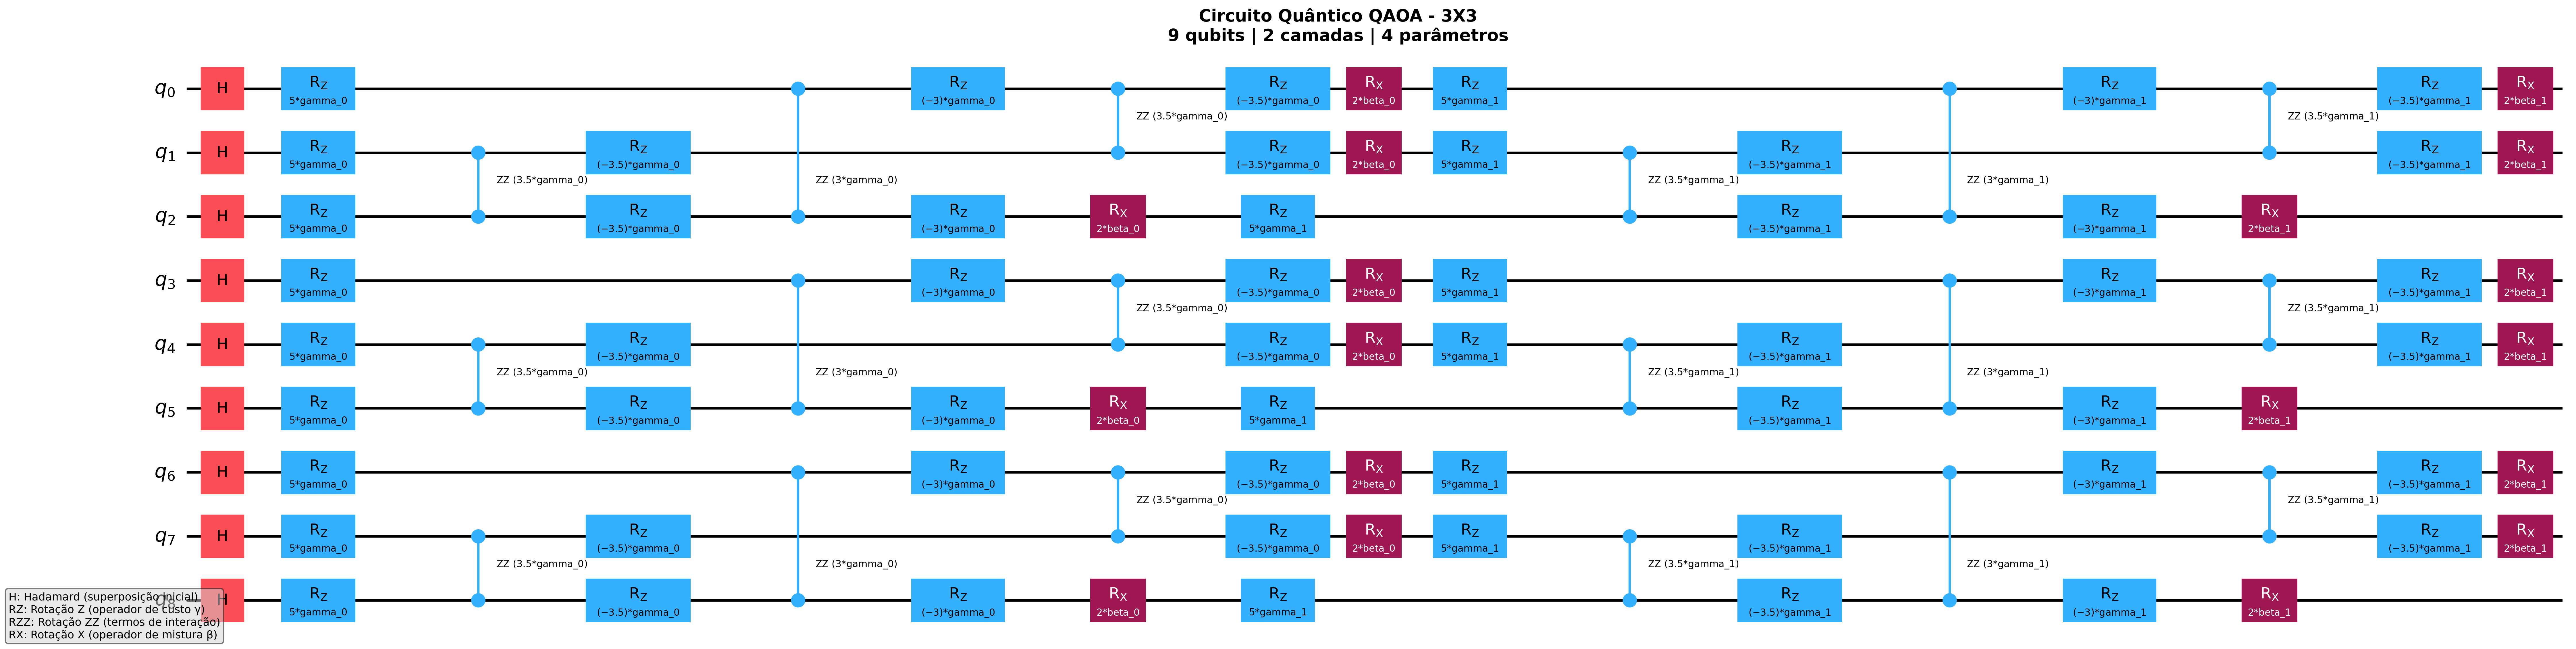
\includegraphics[width=0.95\linewidth]{quantum_circuit_3x3_9qubits_2layers_20250813_095137.png}
\caption{Exemplo de circuito QAOA (2 camadas) para grid 3x3 (9 qubits).}
\end{figure*}

\subsection*{Discussão dos resultados}
Os experimentos revelam comportamentos característicos do QAOA para este problema:
\begin{enumerate}
\item \textbf{Escalabilidade}: O tempo computacional cresce superlinearmente com o tamanho da grade devido à complexidade dos circuitos quânticos resultantes.
\item \textbf{Trade-offs}: Soluções com alta probabilidade frequentemente apresentam penalidades de esteira não-nulas, indicando que o ótimo global pode ser difícil de alcançar.
\item \textbf{Profundidade do \textit{ansatz}}: Maior profundidade $p$ melhora a qualidade das soluções mas aumenta drasticamente o custo computacional.
\item \textbf{Convergência}: A inicialização aleatória dos parâmetros pode levar a mínimos locais diferentes em execuções distintas.
\end{enumerate}

Cenários pequenos (até 3x3) permitem análise detalhada do compromisso entre benefício individual e penalidades coletivas, servindo como validação conceitual antes da extensão para problemas maiores.

\section{Conclusões}

Este trabalho apresentou uma formulação completa de QAOA para otimização de layout de fazendas eólicas considerando efeitos de esteira direcionais. As principais contribuições incluem:

\textbf{Contribuições metodológicas:} (i) Adaptação do problema de otimização de layout eólico para plataformas de computação quântica compatíveis com hardware IBM e similares via framework Qiskit; (ii) modelagem QUBO que captura adequadamente o trade-off entre benefícios individuais e penalidades coletivas de esteira; (iii) implementação configurável permitindo exploração sistemática de cenários.

\textbf{Resultados experimentais:} Demonstramos a viabilidade conceitual do QAOA para grades até 4x4, com convergência consistente e capacidade de encontrar soluções de alta qualidade. O algoritmo captura adequadamente o compromisso fundamental entre maximização de benefícios e minimização de interferências.

\textbf{Limitações identificadas:} (i) Escalabilidade, na simulação clássica, limitada pelo crescimento exponencial do número de estados possíveis; (ii) sensibilidade à inicialização de parâmetros e profundidade do \textit{ansatz}; (iii) necessidade de múltiplas execuções para garantir convergência ao ótimo global; (iv) modelo de esteira simplificado com decaimento linear, que não captura adequadamente a física real dos efeitos de esteira, incluindo expansão radial, variações de velocidade do vento, e interações turbulentas complexas presentes em modelos como Jensen ou Gaussian.

\textbf{Trabalhos futuros:} (i) Incorporação de modelos de esteira mais realistas (Jensen, Park) e propagação diagonal; (ii) desenvolvimento de estratégias de inicialização informadas e mixers personalizados; (iii) benchmarking sistemático contra algoritmos clássicos (algoritmos genéticos, simulated annealing); (iv) avaliação em hardware quântico real considerando ruído e limitações de conectividade; (v) extensão para restrições operacionais complexas (manutenção, acesso, aspectos ambientais).

O código desenvolvido está disponível publicamente em \texttt{https://github.com/vinirn/qaoa\_wind}.

\ifdef{\anonversion}{
  % Seção de agradecimentos omitida na versão anônima
}{
  \section*{Agradecimentos}
  O autor agradece à Universidade Federal Rural do Semi-Árido pelo apoio profissional e logístico. Este trabalho é dedicado à memória do prof. Liacir dos Santos Lucena.
}

\begin{thebibliography}{99}
\bibitem{GWEC2017}
Global Wind Energy Council, ``Global Wind Reports,'' 2024. Disponível em: https://www.gwec.net/reports/globalwindreport (acesso em agosto de 2025).

\bibitem{IRENA2017}
International Renewable Energy Agency (IRENA), ``Renewable Power Generation Costs in 2017,'' 2018. Disponível em: https://www.irena.org/publications/2018/Jan/Renewable-power-generation-costs-in-2017 (acesso em agosto de 2025).

\bibitem{Jensen1983}
N. O. Jensen, ``A Note on Wind Generator Interaction,'' Risø-M-2411, Risø National Laboratory, 1983.

\bibitem{Barthelmie2009}
R. J. Barthelmie et al., ``Modelling and measuring flow and wind turbine wakes in large wind farms offshore,'' Wind Energy, 12(5):431--444, 2009.

\bibitem{Kagemoto2024}
H. Kagemoto, ``Possible application of quantum computing in the field of ocean engineering: optimization of an offshore wind farm layout with the Ising model,'' Journal of Ocean Engineering and Marine Energy, 10:773--782, 2024.

\bibitem{Kochenberger2014}
G. Kochenberger et al., ``The unconstrained binary quadratic programming problem: a survey,'' Journal of Combinatorial Optimization, 28(1):58--81, 2014.

\bibitem{Glover2018}
F. Glover, G. Kochenberger, Y. Du, ``Quantum bridge analytics I: a tutorial on formulating and using QUBO models,'' 4OR, 17(4):335--371, 2019.

\bibitem{Farhi2014}
E. Farhi, J. Goldstone, S. Gutmann, ``A \textit{Quantum Approximate Optimization Algorithm},'' arXiv:1411.4028, 2014.

\bibitem{QiskitAlgorithms}
Qiskit Community, ``Qiskit Algorithms Documentation,'' 2024. Disponível em: https://qiskit.org/ecosystem/algorithms/ (acesso em agosto de 2025).

\bibitem{QiskitCommunity2017}
Qiskit Community, ``Qiskit: An Open-Source Framework for Quantum Computing,'' 2017. DOI: 10.5281/zenodo.2562110. Disponível em: https://github.com/Qiskit/qiskit (acesso em agosto de 2025).

\bibitem{Preskill2018}
J. Preskill, ``Quantum computing in the NISQ era and beyond,'' Quantum, 2:79, 2018.

\bibitem{Cerezo2021}
M. Cerezo et al., ``Variational quantum algorithms,'' Nature Reviews Physics, 3(9):625--644, 2021.
\end{thebibliography}


\end{document}
